\documentclass[12pt,a4paper]{article}
\usepackage{geometry}
\usepackage{graphicx}
\usepackage{amsmath}
\usepackage{hyperref}
\usepackage{enumitem}
\usepackage{fancyhdr}
\usepackage{xcolor}

\geometry{left=2.5cm,right=2.5cm,top=2.5cm,bottom=2.5cm}

\pagestyle{fancy}
\fancyhf{}
\rhead{Confidential - MedTime Disclosure}
\lhead{AI4S-PAT-003}
\cfoot{\thepage}

\title{\textbf{Technical Disclosure Book} \\ \large SYSTEM AND METHOD FOR TOPOLOGICAL CONSISTENCY ENFORCEMENT IN LONGITUDINAL EVENT EXTRACTION}
\author{Internal Ref: AI4S-PAT-003}
\date{\today}

\begin{document}

\maketitle

\section{Technical Field}
The present invention relates to the field of Natural Language Processing (NLP) and Clinical Informatics, specifically to a \textbf{Generate-Verify-Project (GVP)} architecture for ensuring causal and temporal logic consistency in large-scale unstructured data extraction.

\section{Background and Technical Problem}

\subsection{The Technical Defect}
In processing ``Longitudinal Data'' (e.g., Electronic Health Records, Financial Logs), existing sequence-to-sequence models (LLMs) exhibit a specific defect: \textbf{``Temporal Hallucination''}.
\begin{itemize}
    \item \textbf{Root Cause:} Standard Self-Attention mechanisms encode position ($PE$) but do not encode directed graph topology ($G_{time}$).
    \item \textbf{Manifestation:} generated events frequently violate physical causality (e.g., \textit{Surgery} timestamped after \textit{Discharge}, or \textit{Diagnosis} timestamped before \textit{Symptom Onset}).
    \item \textbf{Failure Mode:} On complex clinical benchmarks (MedTime-CN), state-of-the-art models (e.g., Qwen-72B) achieve only \textbf{28.2\% F1} in Zero-Shot settings due to these topology violations.
\end{itemize}

\subsection{Limitation of Prior Art}
\begin{itemize}
    \item \textbf{Rule-based Systems:} Brittle, cannot handle linguistic variety (Recall $< 40\%$).
    \item \textbf{Standard SFT (Supervised Fine-Tuning):} Fits language statistics but not logic; requires massive annotated data.
    \item \textbf{RLHF:} Expensive human feedback, hard to optimize for discrete logic constraints.
\end{itemize}

\section{Technical Solution: GVP Architecture}

The invention proposes a modular \textbf{Neuro-Symbolic System} comprising three coupled processing units.

\subsection{System Architecture}

The core logic relies on Test-Time Projection to enforce topological constraints.

\begin{figure}[h]
    \centering
    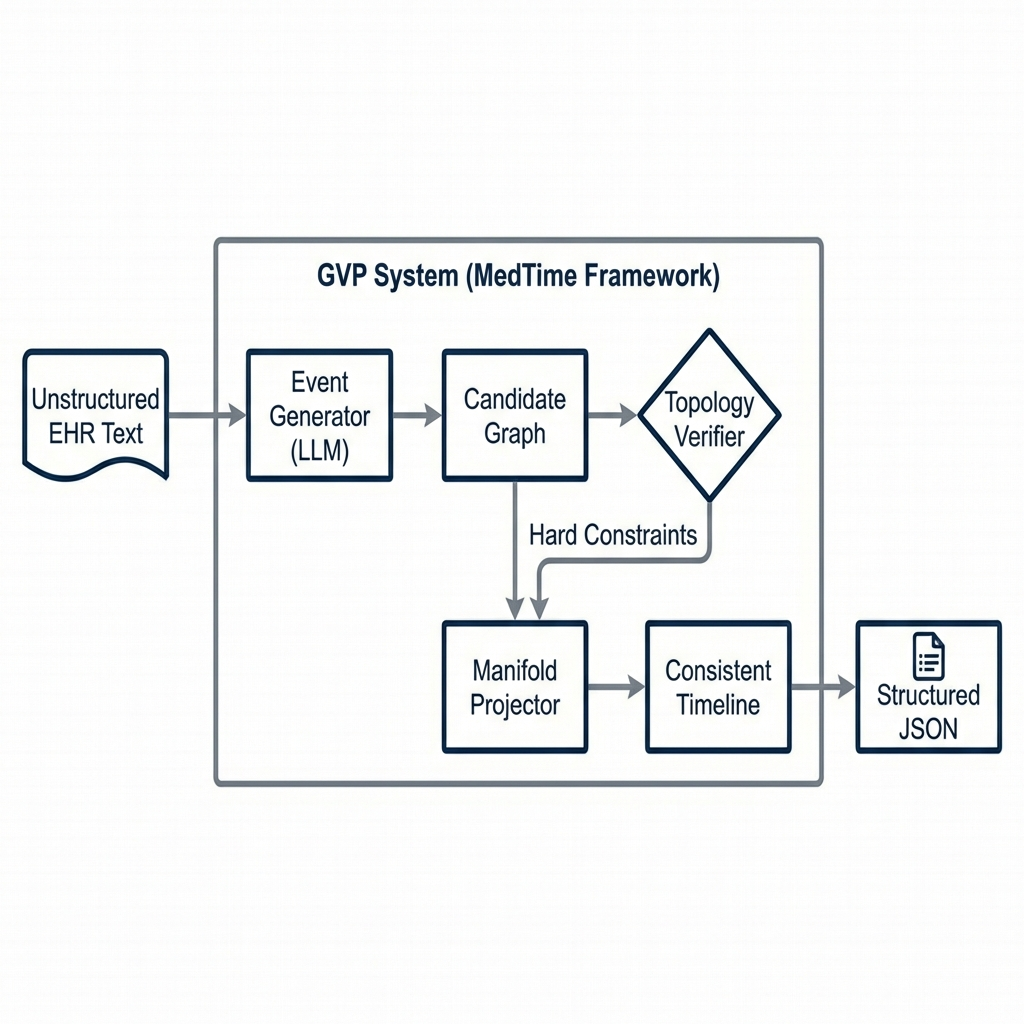
\includegraphics[width=0.9\textwidth]{figs/medtime_architecture.png}
    \caption{System Architecture Diagram of the MedTime GVP Framework.}
    \label{fig:architecture}
\end{figure}

\subsection{Key Modules}

\begin{enumerate}
    \item \textbf{Module 1: Event Generator ($\mathcal{G}$)}
    \begin{itemize}
        \item \textbf{Function:} Extracts raw event mentions $(e, t)$ from unstructured text.
        \item \textbf{Implementation:} A finetuned Transformer model optimized for ``Recall'' rather than Precision. It generates a ``Candidate Graph'' $G_{cand}$ which may contain logic errors.
    \end{itemize}
    
    \item \textbf{Module 2: Topology Verifier ($\mathcal{V}$)}
    \begin{itemize}
        \item \textbf{Function:} A discriminative model (Logic Critic) that scores the validity of event pairs.
        \item \textbf{Mechanism:} It does not predict text. It takes pairs $(e_i, e_j)$ and predicts a relation $R \in \{<, >, =\}$.
        \item \textbf{Output:} A formulation of ``Hard Constraints'' (e.g., $t_{admission} \le t_{surgery} \le t_{discharge}$).
    \end{itemize}
    
    \item \textbf{Module 3: Manifold Projector ($\mathcal{P}$)}
    \begin{itemize}
        \item \textbf{Function:} \textbf{Core Innovation}. A differentiable optimization layer (or discrete search) that projects the flawed output of $\mathcal{G}$ onto the ``Valid Manifold'' defined by $\mathcal{V}$.
        \item \textbf{Hardware Implementation:} This projection occurs at \textbf{Inference Time} (Test-Time) without retraining the large model.
        \item \textbf{Algorithm:} Solves: $\hat{y} = \arg\min_{y} ||y - \mathcal{G}(x)|| \text{ s.t. } \mathcal{V}(y) = \text{Valid}$.
    \end{itemize}
\end{enumerate}

\section{Technical Effects (Beneficial Results)}

\begin{enumerate}
    \item \textbf{Solution to Temporal Hallucination:}
    \begin{itemize}
        \item By explicitly enforcing constraints via $\mathcal{P}$, the system eliminates ``impossible timelines''.
        \item \textbf{Metric:} Temporal F1 score improved from 28.2\% (Baseline) to \textbf{84.2\%} (SOTA) on the verified MedTime-CN dataset.
    \end{itemize}

    \item \textbf{Logic-Language Decoupling (Cross-Lingual Transfer):}
    \begin{itemize}
        \item Because ``Time is Universal'' (topology is language-agnostic), the Verifier trained on Chinese logic successfully corrects English errors.
        \item \textbf{Result:} Zero-shot transfer to English (E3C dataset) achieved \textbf{50.0\% F1}, double the baseline (24.6\%).
    \end{itemize}

    \item \textbf{High-Precision Alignment:}
    \begin{itemize}
        \item Mean Absolute Error (MAE) reduced to \textbf{3.2 days}, enabling deployment in critical Clinical Decision Support (CDS) systems where 40-day errors are unacceptable.
    \end{itemize}
\end{enumerate}

\section{Exemplary Embodiments}

\subsection{Embodiment 1: Cloud-Based Clinical API}
\begin{itemize}
    \item \textbf{Input:} Unstructured Medical PDF/Note.
    \item \textbf{Processing:} Parallel generation of events $\to$ GPU-accelerated Constraint Solving (Projector) $\to$ JSON Output.
    \item \textbf{Output:} Structural Timeline for Insurance Audit.
\end{itemize}

\subsection{Embodiment 2: Edge-Device ``Active Correction''}
\begin{itemize}
    \item Deployed on a doctor's tablet. The ``Verifier'' runs locally (lightweight) to flag timeline errors in real-time dictation (``Doctor, you said discharge was before surgery?'').
\end{itemize}

\section{Claims (Draft Points)}

\begin{enumerate}
    \item \textbf{A Method} for extracting temporally consistent event sequences, comprising:
    \begin{itemize}
        \item Generating a set of candidate events utilizing a generative probabilistic model;
        \item Constructing a topological constraint graph via a discriminative verifier model;
        \item Projecting said candidate events onto a valid solution space defined by said constraint graph to minimize a temporal logic loss.
    \end{itemize}

    \item \textbf{The Method of Claim 1}, wherein the projection is performed at inference time utilizing a constrained optimization algorithm.

    \item \textbf{A System} comprising a processor configured to execute the method of claim 1, specifically adapted to process Electronic Health Records (EHR).
\end{enumerate}

\end{document}
